\documentclass[12pt]{article}
\usepackage{geometry}
\geometry{legalpaper, landscape, margin=0in}
\pagestyle{empty}
\usepackage{amssymb, amsmath, graphicx, wasysym, multirow, epsf, tikz, cancel, hyperref, marvosym, mathtools, amsthm, dcolumn,cases, array}
\usepackage{longtable}

\setlength{\parindent}{0pt} % No indents

\newcommand{\ds}{\displaystyle}
\newcommand{\R}{{\mathbb R}}
\newcommand{\Q}{{\mathbb Q}}
\newcommand{\Z}{{\mathbb Z}}
\newcommand{\N}{{\mathbb N}}
\newcommand{\C}{{\mathbb C}}
\DeclareMathOperator{\Ap}{Ap}
\DeclareMathOperator{\PF}{PF}

\begin{document}
\begin{center}
\begin{longtable}{ |c|c|c|c|c|c|c|c|c| } 
 \hline
  & $S=\left\langle \frac{F+1}{2},\dots,F-4\right\rangle$ & $I$ & $|\lambda(S)|$ & $|\lambda(T)|$ & $F(S)$ & $m(S)$ & $g(S)$ & $GPF(S)$ \\ 
 \hline
 1.1 & $\langle 10,11,12,13,14,15\rangle$ & $\{1,16,18\},\{2,16,17\}$ & 37 & 35 & 19 & 10 & 13 & 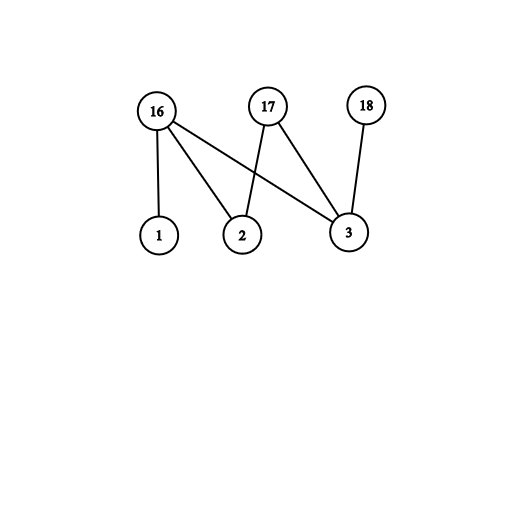
\includegraphics[height=2in]{Table/graph1.1.png}\\
 \hline
 

 1.2 & $\langle 9,10,11,12,13\rangle$ & $\{1,14,16\},\{2,14,15\}$ & 32 & 31 & 17 & 9 & 12 & 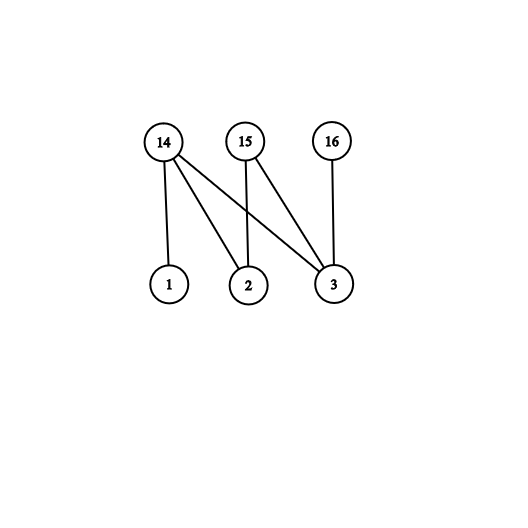
\includegraphics[height=2in]{Table/graph1.2.png}\\
 \hline
 \end{longtable}
\end{center}

\begin{center}
\begin{longtable}{ |c|c|c|c|c|c|c|c|c| } 
 \hline
  & $S$ & $I$ & $|\lambda(S)|$ & $|\lambda(T)|$ & $F(S)$ & $m(S)$ & $g(S)$ & $GPF(S)$ \\ 
 \hline
 2.1 & $\langle 10,11,12,13,14,17\rangle$ & $\{1,15,18\},\{3,15,16\}$ & 35 & 34 & 19 & 10 & 13 & 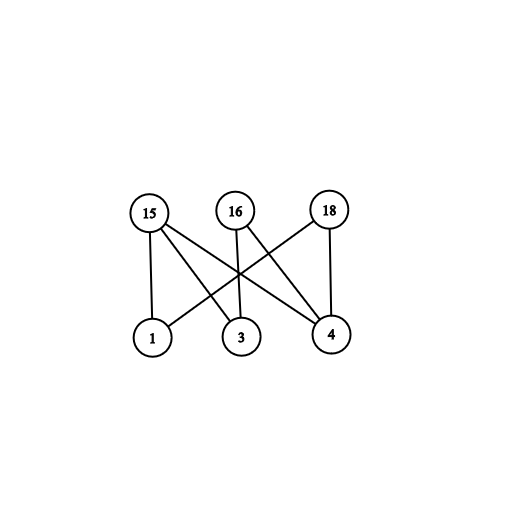
\includegraphics[height=2in]{Table/graph2.1.png} \\
\hline
 2.2 & $\langle11,12,13,14,15,17,20\rangle$ & $\{2,16,19\},\{3,16,18\}$ & 38 & 37 & 21 & 11 & 14 &  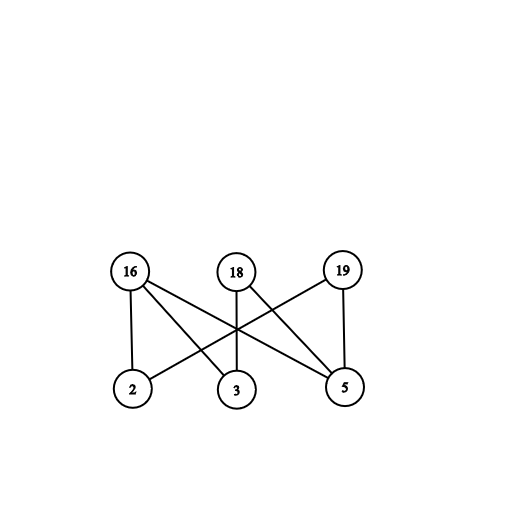
\includegraphics[height=2in]{Table/graph2.2.png}\\
\hline
 2.3 & $\langle12,13,14,15,16,17,20,23\rangle$ & $\{1,18,21\},\{3,18,19\},\{1,11,18,21\},\{3,11,18,19\}$ & 41 & 40 & 22 & 12 & 15 & 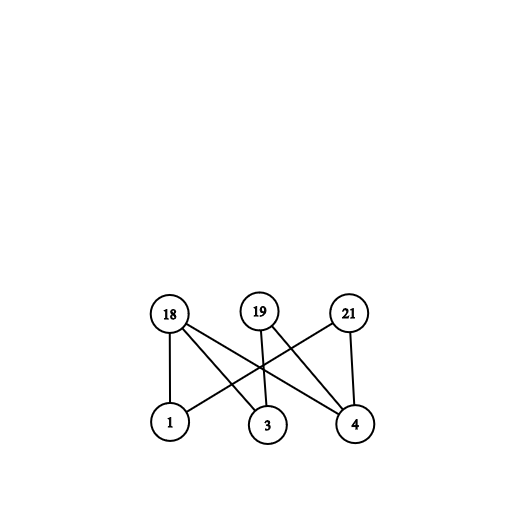
\includegraphics[height=2in]{Table/graph2.3.png} \\
\hline


 2.4 & $\langle12,13,14,15,16,17,18,23\rangle$ & $\{1,19,21\},\{2,19,20\},\{1,11,19,21\},\{2,11,19,20\}$ & 43 & 41 & 22 & 12 & 15 &  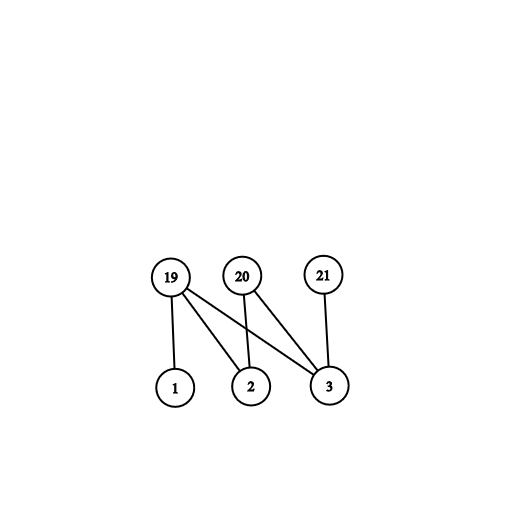
\includegraphics[height=2in]{Table/graph2.4.png} \\
\hline
\end{longtable}
\end{center}
\end{document}